
%(BEGIN_QUESTION)
% Copyright 2008, Tony R. Kuphaldt, released under the Creative Commons Attribution License (v 1.0)
% This means you may do almost anything with this work of mine, so long as you give me proper credit

%Sketch a circuit whereby two loop-powered pressure transmitters send signals to two isolated channels on a datalogger, a device that records electronic signals over long periods of time.  Include one DC power supply in your circuit, along with any other components necessary to make the two 4-20 mA loops work:

Tegn en krets der to trykktransmittere sender signal til to forskjellige kanaler på en datalogger, en komponent som tar opp electroniske signaler over tid. Ta med strømforsyning og eller andre komponenter som trengs for å få kretsen til å fungere. 


$$\includegraphics[width=15.5cm]{i02672x01.eps}$$

\vfil 

\underbar{file i02672}
\eject
%(END_QUESTION)





%(BEGIN_ANSWER)

This is a graded question -- no answers or hints given!

%(END_ANSWER)





%(BEGIN_NOTES)

A good problem-solving technique to apply here is sketching the directions of current through each device (based on its voltage polarity marks and whether it is a {\it load} or a {\it source}).  Then, we will know how the wires must connect in order to keep all the arrows facing the same direction in series loops:

\vskip 10pt

This is just one possible solution:

$$\includegraphics[width=15.5cm]{i02672x02.eps}$$

150 $\Omega$ is the {\it maximum} resistance value practical in this circuit, due to the upper limit of 3 volts on the datalogger.  This, of course, makes the calibrated range of measurement 0.6 volts to 3.0 volts between the datalogger terminals.

%INDEX% Pictorial circuit review (4-20 mA loop)

%(END_NOTES)


